\UseRawInputEncoding
\documentclass{scrartcl}
\usepackage[utf8]{inputenc}
\usepackage{color}
\usepackage{csquotes}
\usepackage{graphicx}
\usepackage{enumitem}
\usepackage{lscape}
\usepackage{booktabs}
\usepackage{hyperref}
\usepackage{float}
\usepackage{xcolor}


\setcounter{secnumdepth}{0}

\title{Image classification with SVM}
\author{Andrea Portscher, Juan Pablo Stumpf, Philip Wille}

\begin{document}
\maketitle

\section{Introduction}
For this project we implemented an image classifier using three different feature extraction approaches: Scale-invariant feature transform (SIFT), Speeded up robust features (SURF) and Histogram of Gradients (HOG). First, we prepared an image dataset containing five different image classes, each comprising training and testing data. After extracting features using the above algorithms, we trained a Support-Vector Machine (SVM) and testetd, how well it was able to classify images.
\section{Approaches}
In the following section we will shortly explain the functionality of the feature extraction algorithms we applied to the dataset - namely SIFT, SURF and HOG.
In general, feature extraction algorithms work in three steps\cite{bay2006}:
\begin{enumerate}
  \item They select interest points at distinctive locations, such as corners.
  \item The neighbourhood of the interest points is represented by a feature vector.
  \item The descriptor vectors are matched between different images.
\end{enumerate}

\subsection{SIFT}
\subsection{SURF}
SURF is based on similar properties as SIFT but is - as the name already takes away - faster and more robust. Unlike SIFT, the SURF algorithm is currently still patented and can therefore only be used by including the \texttt{opencv\_contrib} package\footnote{https://github.com/opencv/opencv\_contrib} and allowing non-free algorithms.

\subsection{HOG}
\section{Implementation}
\subsection{Data}
The image data we used stems from the Caltech-256 Image Set\footnote{http://www.vision.caltech.edu/Image\_Datasets/Caltech256/, accessed on the 22nd of December 2020}, which consists of 256 sets of images of a certain class. We randomly selected 5 of these, namely: cactus, dice, raccoon, spaghetti and sushi. The preaparation of the image data was comprised of the following steps, which we implemented in the file \texttt{utils.py}:
\begin{itemize}
  \item All images were resized to the same size, converted to grayscale and normalized (which removes noise from the image).
  \item All images are associated with a label (their image class).
  \item The images are split into a training set (80\% of images per class) and a testing set (20\% of images).
\end{itemize}

\subsection{Pipeline}
We use a pipeline\footnote{https://scikit-learn.org/stable/modules/generated/sklearn.pipeline.Pipeline.html} which sequentially applies a list of transforms and a final estimator.
In our case the transformers are the application of the respective feature extractor and finally the SVM.
The SIFT and SURF transformers are initialized in the same manner: After the features have been extracted, they are clustered.
In this step we used the MiniBatchKMeans clustering algorithm\footnote{https://scikit-learn.org/stable/modules/generated/sklearn.cluster.MiniBatchKMeans.html}. We used the Elbow Method to approximate the ideal size for K.
This approach works by simply calculating and plotting the distortions as a function of the number of clusters. Then the "elbow" of the graph - meaning the point in which the number of distortions starts to decrease too slowly to justify the additional cost of an increase in the number of clusters. The resulting graph for SIFT can be seen on the following figure. On this base we chose the value 500. 
\begin{center}
  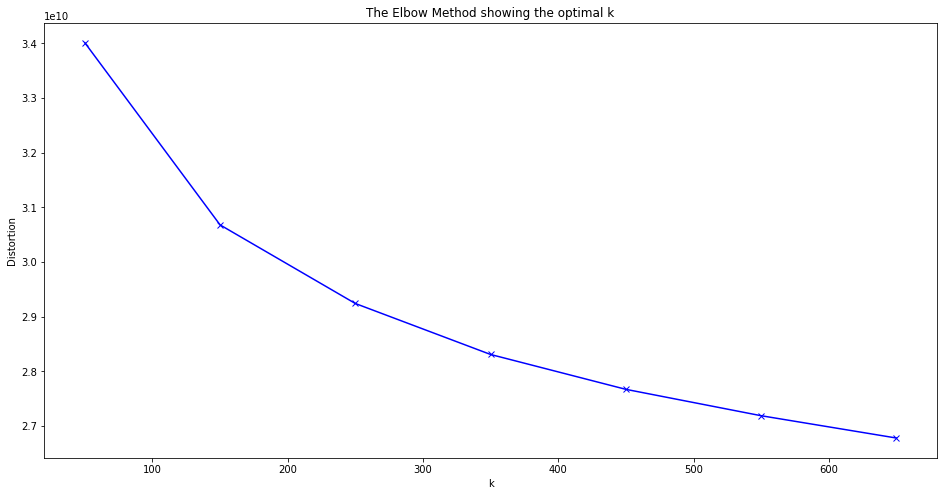
\includegraphics[scale=0.3]{img/kmeans-sift}
\end{center}
After having fitted the MiniBatchKMeans, the transformation begins and histograms are generated.
The next step in the pipeline is the training of the SVM. We chose the LinearSVC algorithm provided by the \texttt{sklearn} library\footnote{https://scikit-learn.org/stable/modules/generated/sklearn.svm.LinearSVC.html}.


\section{Discussion of Results}
In order to be able to evaluate our results we calculated the precision and recall and generated confusion matrices


\bibliographystyle{unsrt}
\bibliography{sources}
\end{document}
